\documentclass[tikz,border=8pt]{standalone}
% Style commun des schémas : thème clair / sombre (couleurs des thèmes GitHub), fond transparent.
\usepackage[T1]{fontenc}
\usepackage{tgheros}
\renewcommand{\familydefault}{\sfdefault}
\usepackage{tikz}
\usetikzlibrary{positioning,arrows.meta,calc,fit,backgrounds}
\ifdefined\darktheme
  \definecolor{fg}{HTML}{E6EDF3}  \definecolor{muted}{HTML}{9198A1}
  \definecolor{line}{HTML}{8B949E} \definecolor{boxfill}{HTML}{151B23}
  \definecolor{boxline}{HTML}{3D444D}
  \definecolor{blue}{HTML}{4493F8} \definecolor{orange}{HTML}{DB6D28}
  \definecolor{green}{HTML}{3FB950} \definecolor{red}{HTML}{F85149}
  \definecolor{purple}{HTML}{AB7DF8}
\else
  \definecolor{fg}{HTML}{1F2328}  \definecolor{muted}{HTML}{59636E}
  \definecolor{line}{HTML}{59636E} \definecolor{boxfill}{HTML}{F6F8FA}
  \definecolor{boxline}{HTML}{D1D9E0}
  \definecolor{blue}{HTML}{0969DA} \definecolor{orange}{HTML}{BC4C00}
  \definecolor{green}{HTML}{1A7F37} \definecolor{red}{HTML}{CF222E}
  \definecolor{purple}{HTML}{8250DF}
\fi
\tikzset{
  every node/.style={text=fg, font=\small},
  block/.style={draw=boxline, fill=boxfill, rounded corners=3pt, line width=0.7pt,
                minimum height=11mm, minimum width=30mm, align=center, inner sep=5pt},
  sub/.style={font=\scriptsize, text=muted},
  wire/.style={line width=1pt, -{Stealth[length=2.6mm]}},
  biwire/.style={line width=1pt, {Stealth[length=2.6mm]}-{Stealth[length=2.6mm]}},
  lbl/.style={font=\scriptsize, text=muted, fill=none, inner sep=2pt},
}

\begin{document}
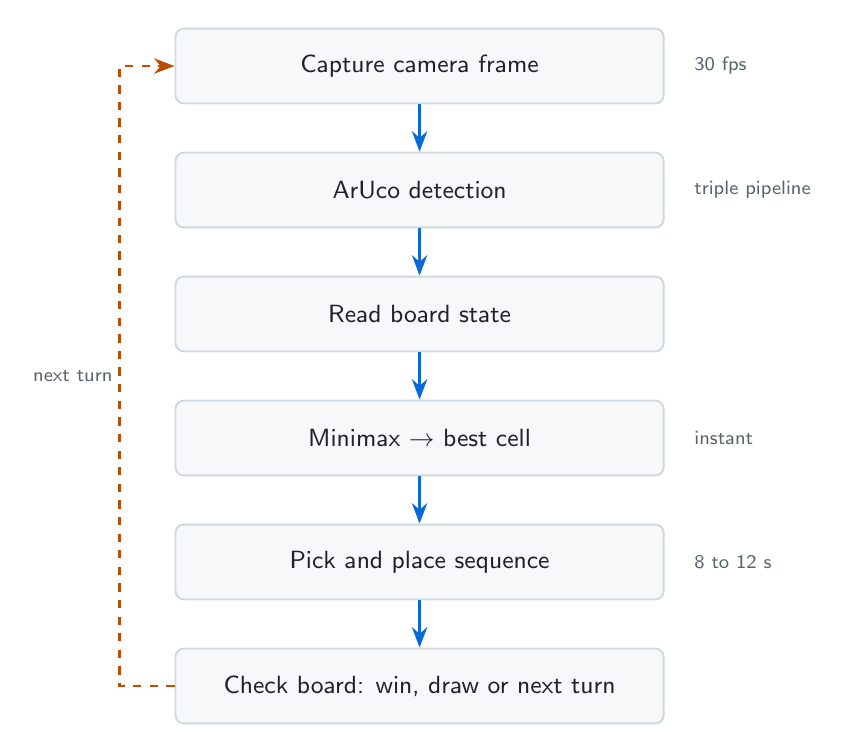
\begin{tikzpicture}[node distance=6mm]
  \tikzset{stage/.style={block, minimum width=62mm, minimum height=9.5mm}}
  \node[stage] (a) {Capture camera frame};
  \node[stage, below=of a] (b) {ArUco detection};
  \node[stage, below=of b] (c) {Read board state};
  \node[stage, below=of c] (d) {Minimax $\rightarrow$ best cell};
  \node[stage, below=of d] (e) {Pick and place sequence};
  \node[stage, below=of e] (f) {Check board: win, draw or next turn};
  \foreach \x/\y in {a/b,b/c,c/d,d/e,e/f} \draw[wire, blue] (\x) -- (\y);
  \foreach \n/\t in {a/30 fps, b/triple pipeline, d/instant, e/8 to 12 s}
    \node[lbl, anchor=west] at ([xshift=3mm]\n.east) {\t};
  \draw[wire, orange, dashed] (f.west) -- ++(-7mm,0) |- node[lbl, left, pos=0.25]{next turn} (a.west);
\end{tikzpicture}
\end{document}
